\documentclass{article}

\usepackage{fancyhdr}
\usepackage{extramarks}
\usepackage{amsmath}
\usepackage{amsthm}
\usepackage{amsfonts}
\usepackage{tikz}
\usepackage{graphicx}
\usepackage{float}
\usepackage{listings}
\usepackage{booktabs}
\usepackage{hyperref}

%\usetikzlibrary{automata,positioning}
\usetikzlibrary{shapes, arrows}

%
% Basic Document Settings
%

\topmargin=-0.45in
\evensidemargin=0in
\oddsidemargin=0in
\textwidth=6.5in
\textheight=9.0in
\headsep=0.25in

\linespread{1.1}

\pagestyle{fancy}
\lhead{\hmwkAuthorName}
\rhead{\hmwkClass\ (\hmwkClassInstructor)}
\cfoot{\thepage}

\lstset{
  caption=\lstname,
  %backgroundcolor=\color{lightgray},
  literate={\$}{{\$}}1,
  breaklines=true,
  basicstyle=\ttfamily\small
}

\DeclareMathOperator*{\argmin}{arg\,min}
\DeclareMathOperator*{\argmax}{arg\,max}
\renewcommand\headrulewidth{0.4pt}
\renewcommand\footrulewidth{0.4pt}

\setlength\parindent{0pt}

\newcommand{\hmwkTitle}{Utilizing reinforcement learning techniques to play Atari's Breakout}
\newcommand{\hmwkDueDate}{November 3, 2015}
\newcommand{\hmwkClass}{Reinforcement Learning}
\newcommand{\hmwkClassInstructor}{Dr. Itamar Arel}
\newcommand{\hmwkAuthorName}{Andrew Messing, Ben Brock, and Cory Walker}

%
% Title Page
%

\title{
    \vspace{2in}
    \textmd{\textbf{\hmwkTitle}}\\
    \normalsize\vspace{0.1in}\small{Due\ on\ \hmwkDueDate}\\
    \vspace{0.1in}\large{\textit{\hmwkClassInstructor}}
    \vspace{3in}
}

\author{\textbf{\hmwkAuthorName}}
\date{}

\renewcommand{\part}[1]{\textbf{\large Part \Alph{partCounter}}\stepcounter{partCounter}\\}

%
% Various Helper Commands
%

% Alias for the Solution section header
\newcommand{\solution}{ \hfill \break \break \textbf{Solution} \hfill \break \break}

\begin{document}

\maketitle

\pagebreak

\begin{abstract}
  Abstract goes here. Ben, could you take care of this?
\end{abstract}

\section{Introduction}
Some type of introduction goes here. Andrew, could you take care of this?

\section{Breakout and feature extraction}
Andrew's section goes here.

\section{Reinforcement learning}
Ben's section goes here.

\section{Deep reinforcement learning}
  While manual feature extraction can result in faster training and potentially better performance, there is a large motivation to be able to learn from general and high dimensional inputs such as video and sound. If we could learn to play Atari games from raw pixels, we could use the same algorithm on an array of games, even games we have never actually played before. \\

  Of course, things are not as simple as creating a state for every possible screen. Since the Atari environment has 128 colors and a 210x160 screen, the number of states resulting from this would be $128^{210 \cdot 160} \approx 1.799\times 10^{70802}$. Even if we reduced the number of colors to 4, we would still have a number with 20,000 digits for the number of states. Furthermore, even if we cut the screen size by a quarter, we would still have $4^{105 \cdot 80} \approx 2.013\times 10^{5057}$ states. \\

  On top of all this, just a single screen in Breakout and many other Atari games is just a partial representation of the game state. The ball could be moving either right or left, which is an important piece of information for scoring points. \\

  Recently Google DeepMind has made progress in this problem space by utilizing convolutional neural networks for estimating the action-value function based on visual input. The rest of this project will describe implementing DeepMind's Double DQN algorithm, an algorithm for which no open-source implementation previously existed.
\subsection{Deep Q network}
  The standard Deep Q network for playing Atari games features around 1.5 million parameters. Each parameter is updated through the following equation:
  \[ \boldsymbol{\theta}_{t+1} = \boldsymbol{\theta}_t+\alpha(Y_t^Q-Q(S_t,A_t;\boldsymbol{\theta}_t))\nabla_{\boldsymbol{\theta}_t}Q(S_t,A_t;\boldsymbol{\theta}_t) \]
  The network is composed of the following stacked sequence of layers:
  \begin{enumerate}
    \item An input layer for the past 4 scaled (84x84) and grayscale snapshots of the screen.
    \item A 2D convolution layer with 32 filters of size 8 and stride 4. The layer uses a ReLU nonlinearity.
    \item A 2D convolution layer with 64 filters of size 4 and stride 2. The layer uses a ReLU nonlinearity.
    \item A 2D convolution layer with 64 filters of size 3 and stride 1. The layer uses a ReLU nonlinearity.
    \item Next we have a fully-connected layer with 512 units. This layer uses a ReLU nonlinearity.
    \item Finally we have another fully-connected layer as the output layer with $|A|$ outputs. This layer uses linear activation.
  \end{enumerate}

\subsection{DQN variations}
  \begin{itemize}
  \item {
      NIPS (late 2013) - original paper from workshop, 24 hour training time
  }
  \item {
      Nature (early 2015) - similar to NIPS, more conservative hyperparameters (7 day training), model freezing
  }
  \item {
      Double DQN (September 2015) - branch from Nature model, attempts to address value overestimates
  }
  \end{itemize}

\subsection{Double DQN formulation}
  \begin{itemize}
    \item max operator means we use same values for action selection and evaluation, want to decouple.
    \item Action-value function has weights $\boldsymbol{\theta}_t$
    \item Target action-value function has weights $\boldsymbol{\theta}_t^-$
    \item After every 10,000 training updates, $\boldsymbol{\theta}_t^- \leftarrow \boldsymbol{\theta}_t$
  \end{itemize}

  \[Y_t^{\textrm{DQN}} \equiv R_{t+1} + \gamma \textcolor{red}{\max_{a} Q(S_{t+1},a;\boldsymbol{\theta}_t^-)} \]
  \[ \Downarrow \]
  \[\boxed{Y_t^{\textrm{DoubleDQN}} \equiv R_{t+1} + \gamma \textcolor{red}{Q(S_{t+1},\argmax_a Q(S_{t+1},a;\boldsymbol{\theta}_t),\boldsymbol{\theta}_t^-)}} \]
  \begin{itemize}
    \item If $\boldsymbol{\theta}_t^- = \boldsymbol{\theta}_t$ (NIPS model), no difference
  \end{itemize}

\subsection{Implementation}
  \begin{itemize}
    \item Nathan Sprague, \href{https://github.com/spragunr/deep_q_rl}{https://github.com/spragunr/deep\_q\_rl}
    \item Circular buffer for 1M replay frames, visualization code, model saving and loading
    \item Already supported NIPS and Nature algorithms.
    \item After some Theano debugging, my fork now supports Double DQN
    \item EC2 g2.2xlarge
    \item Single threaded, CPU bound, 30\% GPU utilization, 8GB replay buffer
  \end{itemize}

\subsection{Results}
  \begin{figure}[H]
    \centering
    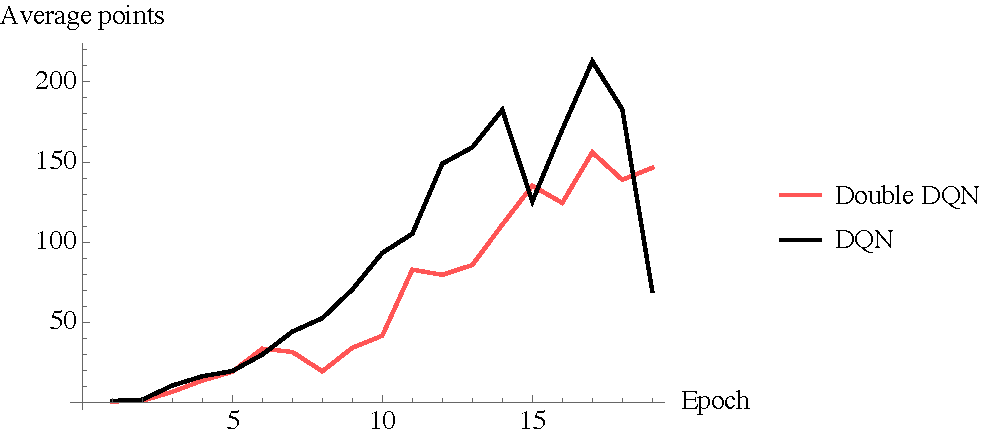
\includegraphics[width=120mm]{dqn_rewardper.pdf}
  \end{figure}
  Each epoch takes about an hour. Stopped after $\sim 20$ hours.\\
  \begin{figure}[H]
    \centering
    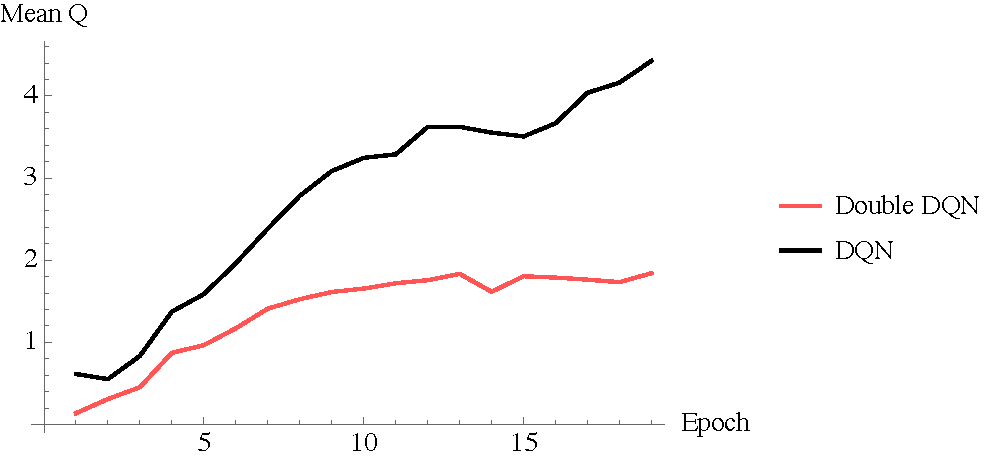
\includegraphics[width=120mm]{dqn_meanq.pdf}
  \end{figure}

\section{Design challenges}
Put design challenges here.

\section{Summary}
A summary goes here.

%\section{Appendix}
%\begin{center}
  %\lstinputlisting{/Users/cwalker32/Documents/LaTeX/ece_517/proj2/et.m}
%\end{center}


\pagebreak

\end{document}
